\documentclass[12pt,a4paper]{jsarticle}
\setlength{\topmargin}{-2.04cm}
\setlength{\oddsidemargin}{-1.04cm}
\setlength{\evensidemargin}{-1.04cm}
\setlength{\textwidth}{18cm}
\setlength{\textheight}{26cm}

\usepackage[latin1]{inputenc}
\usepackage{amsmath}
\usepackage{amsfonts}
\usepackage{amssymb}
\usepackage[dvipdfmx]{graphicx}
\usepackage{listings}
\usepackage{listings,jvlisting}
\usepackage{geometry}

\lstset{
basicstyle={\ttfamily},
identifierstyle={\small},
commentstyle={\smallitshape},
keywordstyle={\small\bfseries},
ndkeywordstyle={\small},
stringstyle={\small\ttfamily},
frame={tb},
breaklines=true,
columns=[l]{fullflexible},
xrightmargin=0zw,
xleftmargin=3zw,
numberstyle={\scriptsize},
stepnumber=1,
numbersep=1zw,
lineskip=-0.5ex
}

\author{来代 勝胤}
\title{モンテカルロ法による面積計算}

\begin{document}
\maketitle
\thispagestyle{empty}
\clearpage
\addtocounter{page}{-1}

\newgeometry{left=15mm,right=15mm,top=15mm,bottom=20mm}
\section{理論}
以下の5つの曲線と、$x=0$、$x=1$、$y=0$が囲む面積を求める。
\begin{eqnarray}
    f(x)=&x\\
    f(x)=&x^2\\
    f(x)=&\cos\left(\frac{\pi}{2}x\right)\\
    f(x)=&\sin\left(\pi x\right) \\
    f(x)=&\exp\left(-x^2\right)
\end{eqnarray}
乱数を用いたモンテカルロ法で面積を評価する。
$n$回目に発生させた乱数を$r^n$として、設定点座標を$\left(r^n, r^{n+1}\right)$で与える。\\
\begin{center}
    設定点の$y$座標          $r^{n+1}$\\
    設定点の$x$座標の関数値 $f\left(r^n\right)$
\end{center}
上記、2式の大小を比較し、$r^{n+1}>f(r^n)$であれば、$S_1$領域、$r^{n+1}<f(r^n)$であれば$S_2$領域に属するものと判断できる。
ここで、設定点を$N$点としたときに、今回の場合においては$S_2$領域に属する設定点の比率から面積を求めることが可能である。\\
\section{解析解}
\subsection{$f\left(x\right)=x$について}
\begin{eqnarray}
    S=\int_0^1f\left(x\right)dx=\left[\frac{1}{2}x^2\right]_0^1=\frac{1}{2}=0.5
\end{eqnarray}
\subsection{$f\left(x\right)=x^2$について}
\begin{eqnarray}
    S=\int_0^1f\left(x\right)dx=\left[\frac{1}{3}x^3\right]_0^1=\frac{1}{3}=0.333\dots
\end{eqnarray}
\subsection{$f\left(x\right)=\cos\left(\frac{\pi}{2}x\right)$について}
\begin{eqnarray}
    S=\int_0^1f\left(x\right)dx=\left[\frac{2}{\pi}\sin\left(\frac{\pi}{2}x\right)\right]_0^1=\frac{2}{\pi}=0.636619\dots
\end{eqnarray}
\subsection{$f\left(x\right)=\sin\left(\pi x\right)$について}
\begin{eqnarray}
    S=\int_0^1f\left(x\right)dx=\left[-\frac{1}{\pi}\cos\left(\pi x\right)\right]_0^1=\frac{2}{\pi}=0.636619\dots
\end{eqnarray}
\subsection{$f\left(x\right)=\exp\left(-x^2\right)$について}
誤差関数$erf(t)$の定義、\\
\begin{eqnarray}
    erf\left(t\right)=\frac{2}{\sqrt{\pi}}\exp\int_0^t\left(-x^2\right)dx
\end{eqnarray}
より、求める解析解は以下のように表すことができる。
\begin{eqnarray}
    S=\int_0^1\exp\left(-x^2\right)=\frac{\sqrt{\pi}}{2}erf\left(1\right)=\frac{\sqrt{\pi}}{2}×0.8427=0.746823\dots
\end{eqnarray}
\section{結果}
今回、パラメータとなる設定点数$N$に関して、$N=5000$と設定し計算を行った。\\
ここで、検討事項である「設定点$N$と面積算出値の関係」を図1に、「面積算出値と解析解との誤差」を図2に示す。
\begin{figure}[htbp]
    \begin{center}
        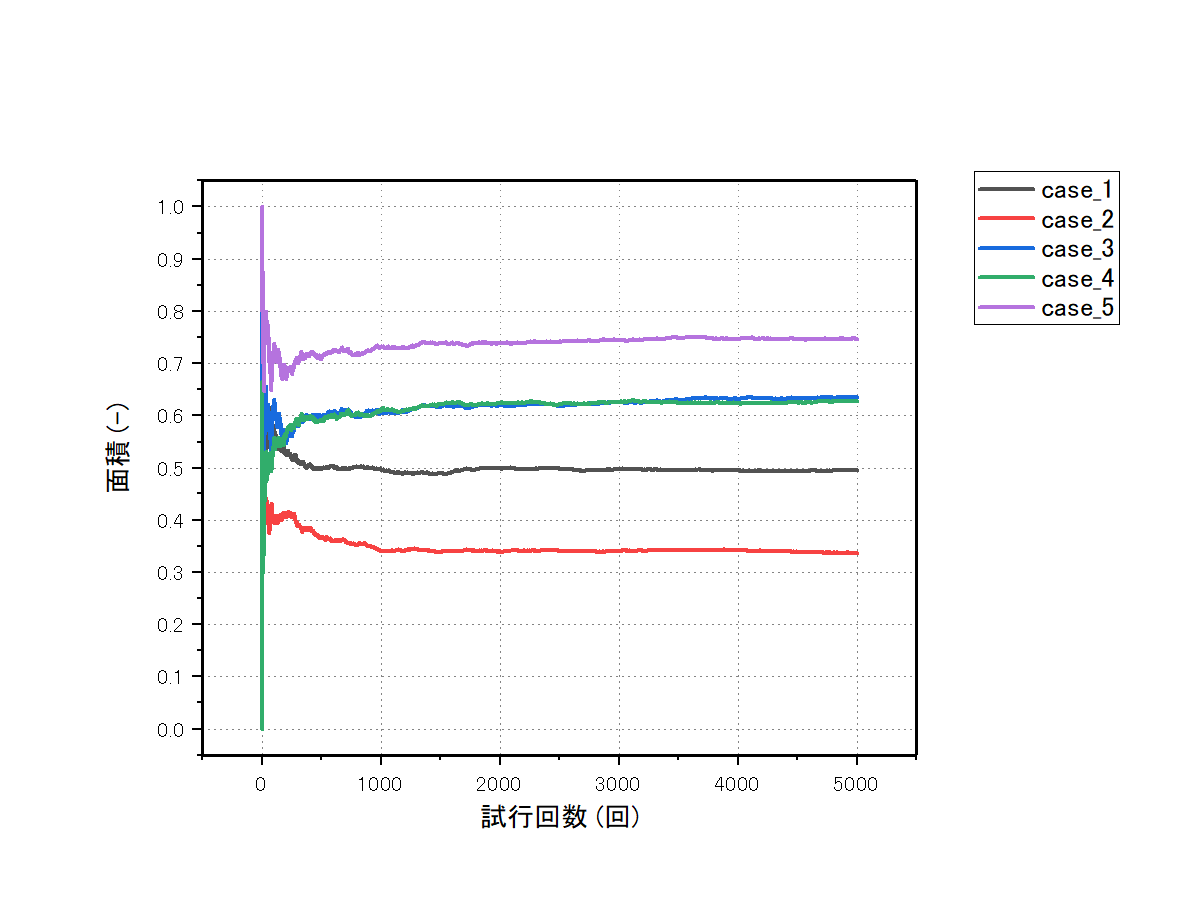
\includegraphics[width=150mm]{Graph/result_0-5000.png}
        \caption{設定点$N$と面積算出値の関係 (0-5000)}
    \end{center}
\end{figure}
\begin{figure}[htbp]
    \begin{center}
        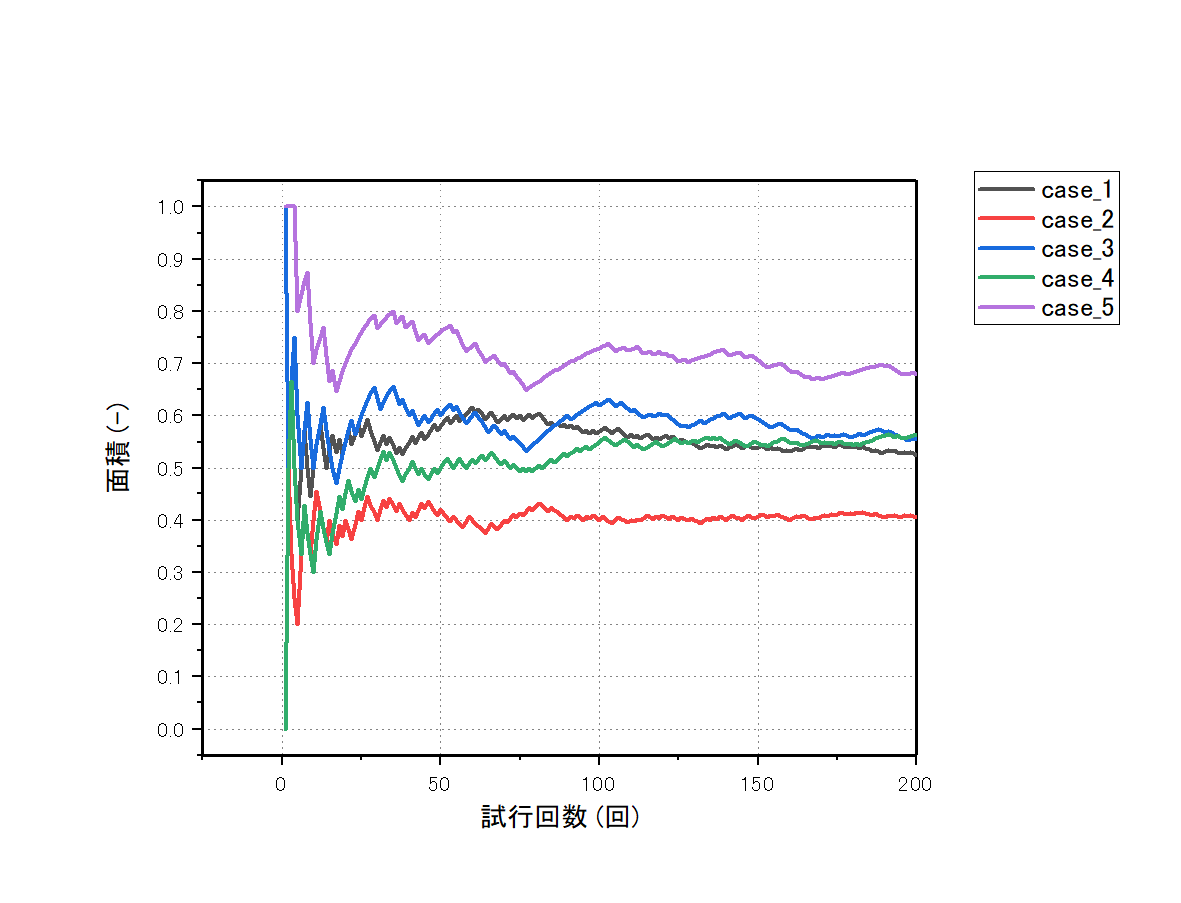
\includegraphics[width=150mm]{Graph/result_0-200.png}
        \caption{設定点$N$と面積算出値の関係 (0-200)}
    \end{center}
\end{figure}
\begin{figure}[htbp]
    \begin{center}
        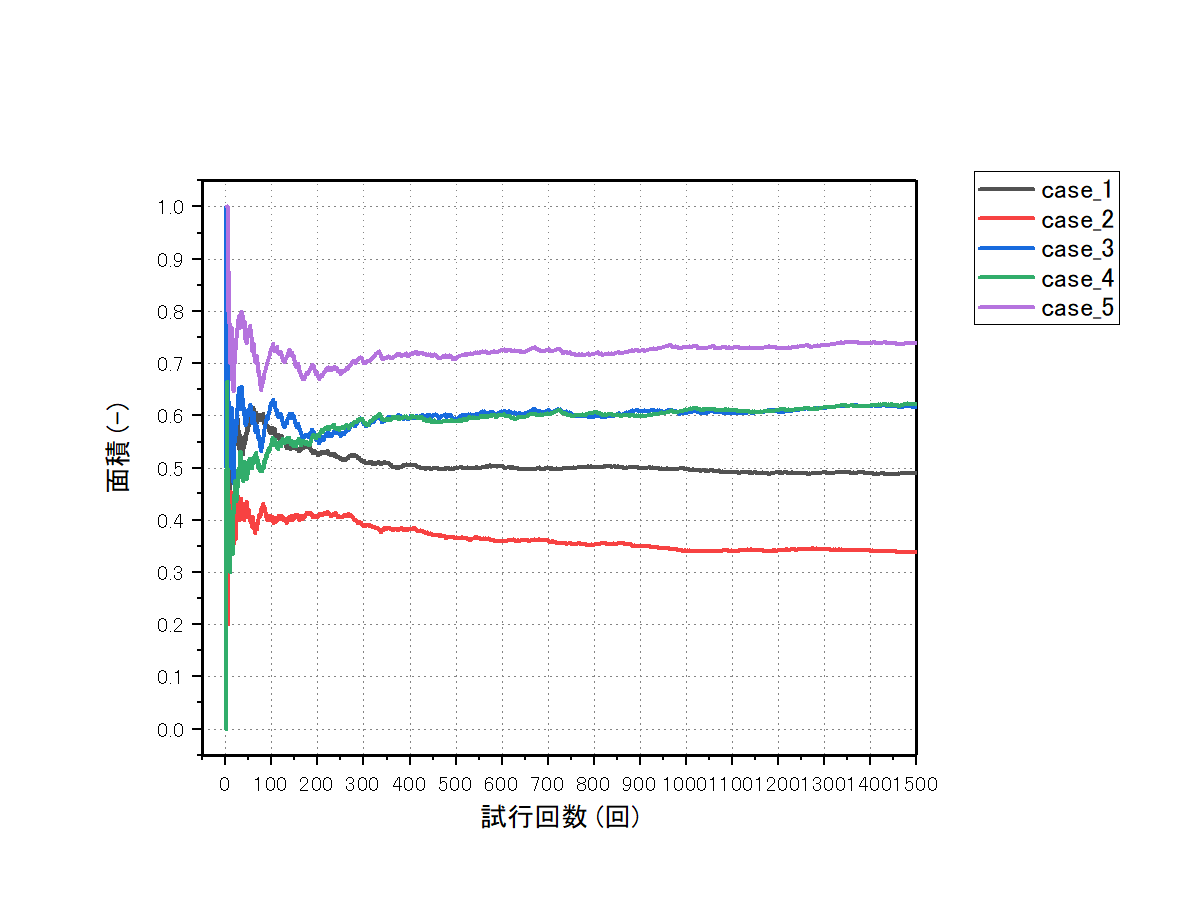
\includegraphics[width=150mm]{Graph/result_0-1500.png}
        \caption{設定点$N$と面積算出値の関係 (0-1500)}
    \end{center}
\end{figure}
\begin{figure}[htbp]
    \begin{center}
        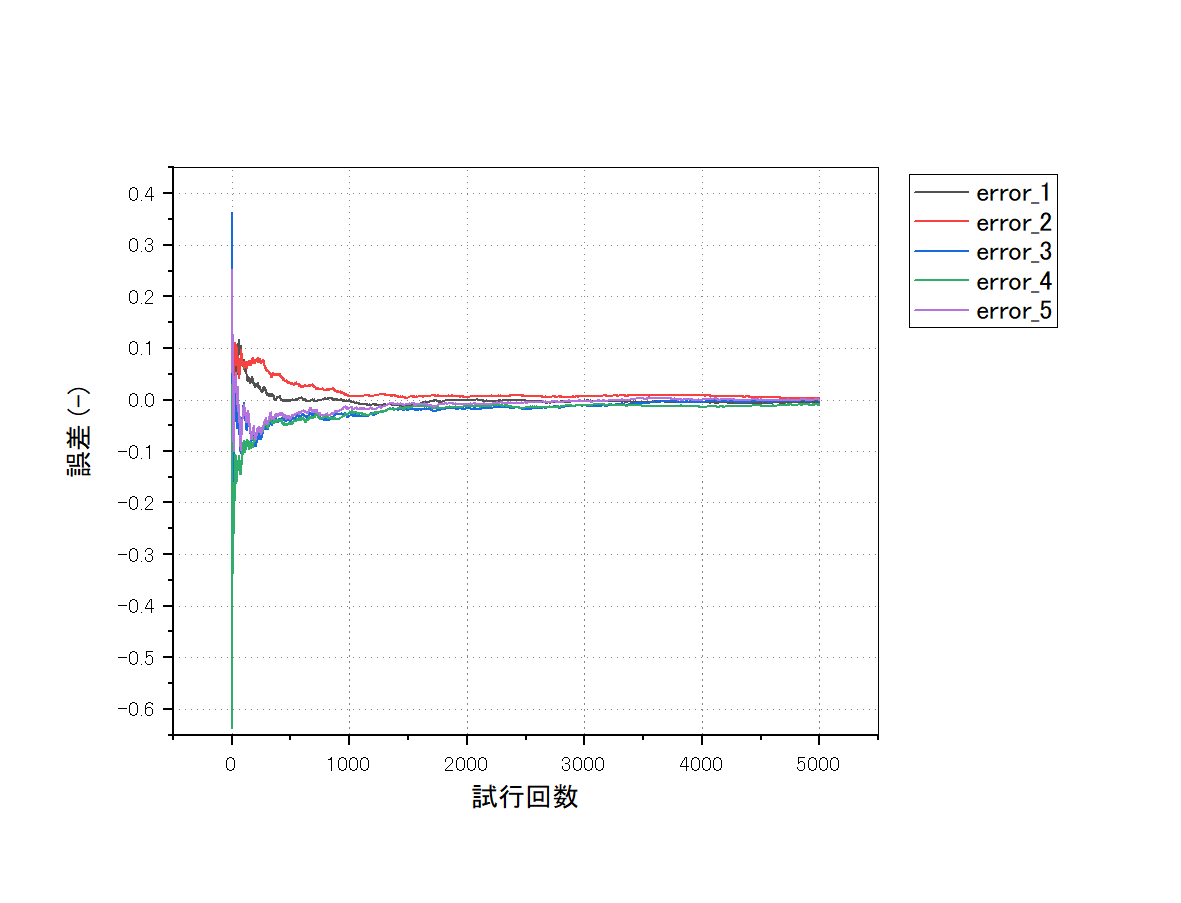
\includegraphics[width=150mm]{Graph/error_0-5000.png}
        \caption{面積算出値と解析解との誤差 (0-5000)}
    \end{center}
\end{figure}
\begin{figure}[htbp]
    \begin{center}
        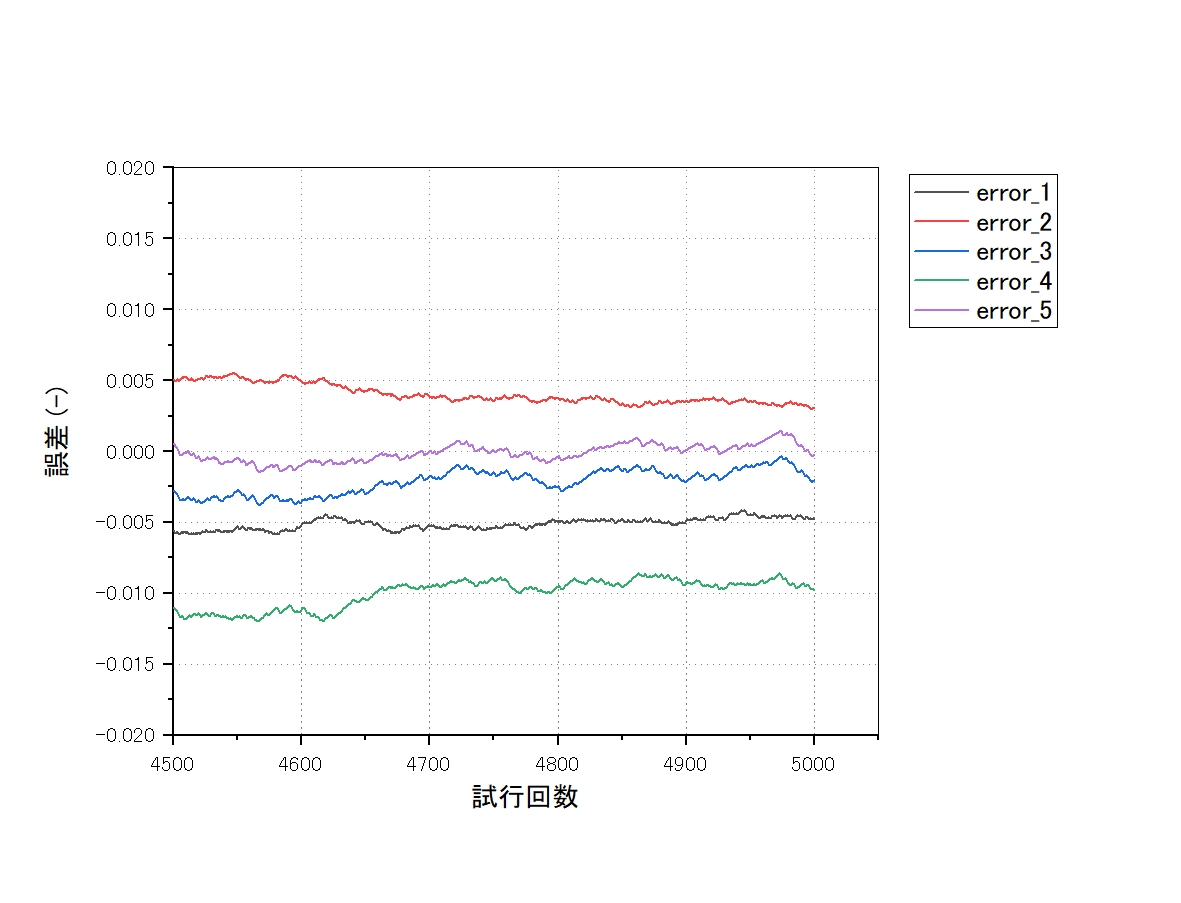
\includegraphics[width=150mm]{Graph/error_4500-5000.png}
        \caption{面積算出値と解析解との誤差 (4500-5000)}
    \end{center}
\end{figure}

\newpage
\section{考察}
まず、「設定点$N$と面積算出値の関係」について考える。
図1をみると、試行回数が大きくなるにつれて一定の値に収束していくことがみれる。
ここで、試行回数が0〜200回および0〜1500回における面積算出値の図をそれぞれ図2、図3に示す。
図2をみると、試行回数が約80回を超えるあたりまでは値が大きく振動していることがみれるが、
その後はある程度の範囲内に値が収まっていることがわかる。\\
しかし、図3をみると約300回を超えたあたりで値に動きがみられ徐々に解析解へ近づいて行くことがわかる。
そして1000回を超えた後、ほぼ一定の値を取り続けている。
また、「面積算出と解析解の誤差」についても同様の傾向が図4〜図5についてみることができる。
試行回数が5000回の時点では誤差は±0.01以内に収まっているため、
ある程度の精度は確保できていると考えられる。\\
式(1)〜(5)について収束速度等に同様の傾向が見られるのは、同じ乱数列を使用したためであると考えられる。
また、試行回数を100000回に設定したところ、誤差は少数第4位のオーダまで縮めることができた。\\
\\
\textbf{試行回数100000回における誤差の出力結果}\\
error1:-3.69995823E-04\\
error2:-6.32345676E-04\\
error3: 5.51223755E-04\\
error4: 4.80234623E-04\\
error5: 2.89857388E-04\\
\\
それ以上の試行回数にした場合も微量ではあるが誤差はより小さくなる傾向がみられた。
しかし、値の算出に必要な時間(プログラムの動作時間)は大きくなったため(今回の場合はファイルへの書き込みに時間を要する)、
必要な値のオーダに応じて試行回数の使いわけが必要であると感じた。\\
今後の研究においても、シミュレーションを行う際に同様の問題が生じると考えられ、
より負荷のかかる処理が必要であるため非常に長い時間が解析に要する場合も考えられる。
目的に応じて適切にパラメータを設定することが重要であると感じた。
\section{プログラム}
今回使用したプログラムを以下に示す。
\small
\begin{lstlisting}
    ! Program Name : report.f90

program main

    implicit none
    integer, parameter :: num = 5000
    integer, parameter :: case = 5
    integer i, j, n
    real x, y, a, b, pi, f_1, f_2, f_3, f_4, f_5
    real f(case),s(case)
    real r(num + 1)
    real area(num + 1, case)
    real dif(num + 1, case)

    !** create random number *********************
    
    integer :: seedsize
    integer, allocatable :: seed(:)
    
    call random_seed(size = seedsize)       
    allocate(seed(seedsize))               
    do j = 1, seedsize
        call system_clock(count = seed(j)) 
    end do
    call random_seed(put = seed(:))         
    
    !********************************************

    pi = 4.0 *atan(1.0)
    ! write(6,*)'pi = ',pi

    call random_number(r)

    do 10 j = 1 ,case
       s(j) = 0
    10 continue

    open(17, file = 'result/result.dat', status='replace')

    do 20 i = 1, num
        x = r(i)
        y = r(i + 1)
    
        f(1) = x                  !case_1
        f(2) = x*x                !case_2
        f(3) = cos(pi / 2.0 * x)  !case_3
        f(4) = sin(pi * x)        !case_4
        f(5) = exp(-x * x)        !case_5

        do 100 j = 1, 5   
            if (f(j) > y) then
                s(j) = s(j) + 1
            end if    
            a = (s(j)/i)
            area(i,j) = a
        100 continue
        20 continue

    do 30 i = 1, num
        write (17,*) i,area(i,1),area(i,2),area(i,3),area(i,4),area(i,5)
    30 continue

    close(17)

    open(18, file= 'result/difference.dat', status='replace')

    f_1 = 1.0/2.0
    f_2 = 1.0/3.0
    f_3 = 2.0/pi
    f_4 = 2.0/pi
    f_5 = sqrt(pi)/2*erf(1.0)

    do 40 i = 1, num
        dif(i,1) = area(i,1) - f_1
        dif(i,2) = area(i,2) - f_2
        dif(i,3) = area(i,3) - f_3
        dif(i,4) = area(i,4) - f_4
        dif(i,5) = area(i,5) - f_5
    40 continue

    do 50 i = 1, num
        write (18,*) i,dif(i,1),dif(i,2),dif(i,3),dif(i,4),dif(i,5)
    50 continue

    close(18)

end program
\end{lstlisting}

\end{document}